\documentclass[a4paper,14pt]{article}
\usepackage[left=2.5cm, right=1.5cm, top=2.5cm, bottom=2.5cm]{geometry}

\usepackage[hidelinks]{hyperref}
\usepackage{titletoc}
\usepackage{titlesec}
\usepackage{titling}

\usepackage[nottoc]{tocbibind}

\setlength\parindent{5ex}
\usepackage[utf8]{inputenc}
\usepackage[russian]{babel}
\usepackage{amsmath,amsthm,amssymb}
\usepackage{mathtext}
\usepackage{amsmath}
\usepackage{graphicx}
\usepackage{longtable}
\usepackage{hyperref}
\usepackage{multicol}
\usepackage{subcaption}
\usepackage[]{algorithm2e}
\usepackage[T1,T2A]{fontenc}

    
\title{\textbf{Композиции алгоритмов для решения задачи регрессии}}
\author{Листопадов Иван Сергеевич, ВМК, 317 группа}
\renewcommand\maketitlehooka{\null\mbox{}\vfill}
\renewcommand\maketitlehookd{\vfill\null}



\begin{document}

\begin{titlingpage}
        \maketitle
    \end{titlingpage}
    
\newpage
    \tableofcontents{}
\newpage


\section{Постановка задачи}
Задача заключается в реализации композиций алгоритмов с целью их применения в прогнозировании цен на недвижимость. Необходимо реализовать подходы Random Forest и Gradient Boosting над решаюшими деревьями, провести ряд экспериментов на данных из соревнования House Sales in King Country, USA, исследовать поведение моделей при различных параметрах.

\section{Обработка данных}
Для удобства работы с данными нужно перевести их в числовой формат. Все столбцы исходной таблицы с данными имеют целый или вещественный тип, за исключением столбца с датой. Для расширения признакового пространства и увеличения многообразия комбинаций признаков колонка с датой была преобразована в 3 колонки с номерами года, месяца и дня. Таким образом, была получена вещественная матрица, которую можно преобразовать в numpy массив.


\section{Необходимые модули}
Прежде чем проводить эксперименты, необходимо реализовать данные алгоритмы. Вся реализация содержится в модуле {ensembles.py} и согласуется с требованиями предоставленными в общем задании.

\section{Модель RandomForest}
\subsection{Структура модели}
Модель RandomForestMSE представляет собой композицию решающих деревьев. Каждое дерево выдаёт некоторое предсказание. Предсказание одного дерева может сильно отличаться от реального значения, однако усреднение предсказаний многих деревьев может приблизить выдаваемый ответ к верному намного ближе. Чтобы этого добиться, нужно правильным образом обучать деревья. Обучив их всех на одном и том же наборе данных, мы породим множество идентичных деревьев, следовательно, необходимо варьировать обучающую выборку для каждого дерева, делая их как можно «уникальнее». Эти выборки будут создаваться путем случайного взятия объекта из общей выборки с возможным повторением. Также в качестве гиперпараметра можно использовать долю используемых признаков при обучении каждым деревом из общего набора признаков.

\begin{figure}[h!]
                \centering
                \begin{subfigure}[b]{1.0\textwidth}
                    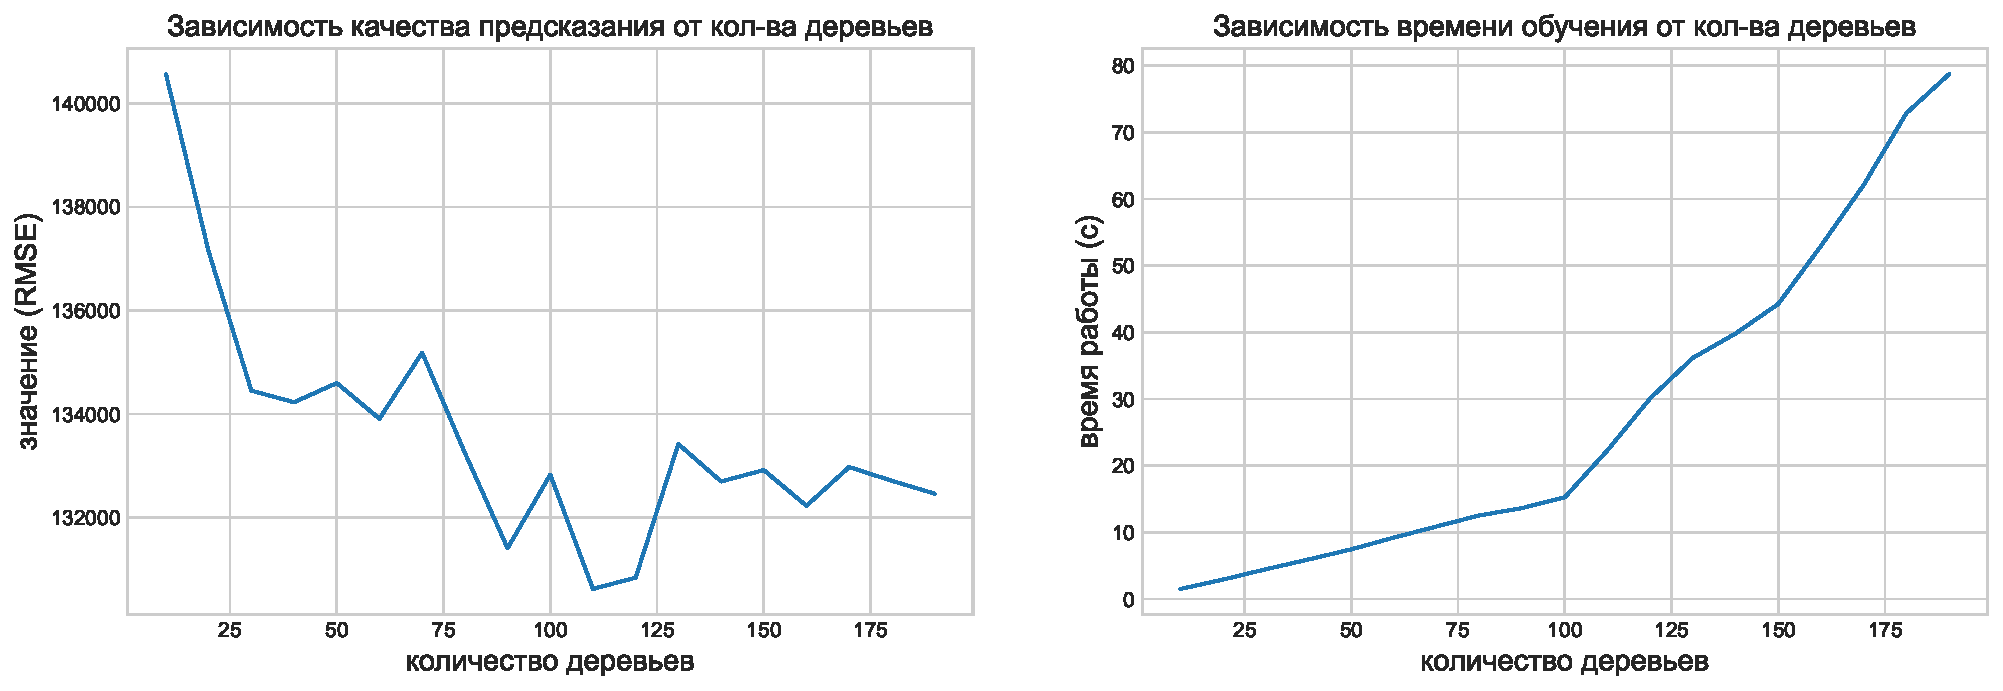
\includegraphics[width=\linewidth]{images/1.1.pdf}
                \end{subfigure}
            \end{figure} \\

\subsection{Влияние числа деревьев на работу модели}
Одним из ключевых параметров модели является количество решающих деревьев, которые используются для прогнозирования. Увеличивая количество деревьев, можно повысить качество предсказания, однако существует порог выше которого качество поднять будет крайне сложно и возможен эффект переобучения. Увеличение количества составляющих в алгоритме требует больше времени на обучение всей модели. Тогда имеет смысл ограничить число деревьев на некотором уровне и не превышать его, чтобы защитить себя от побочных эффектов. Графики выше демострируют это.\\

\begin{figure}[h!]
                \centering
                \begin{subfigure}[b]{1.0\textwidth}
                    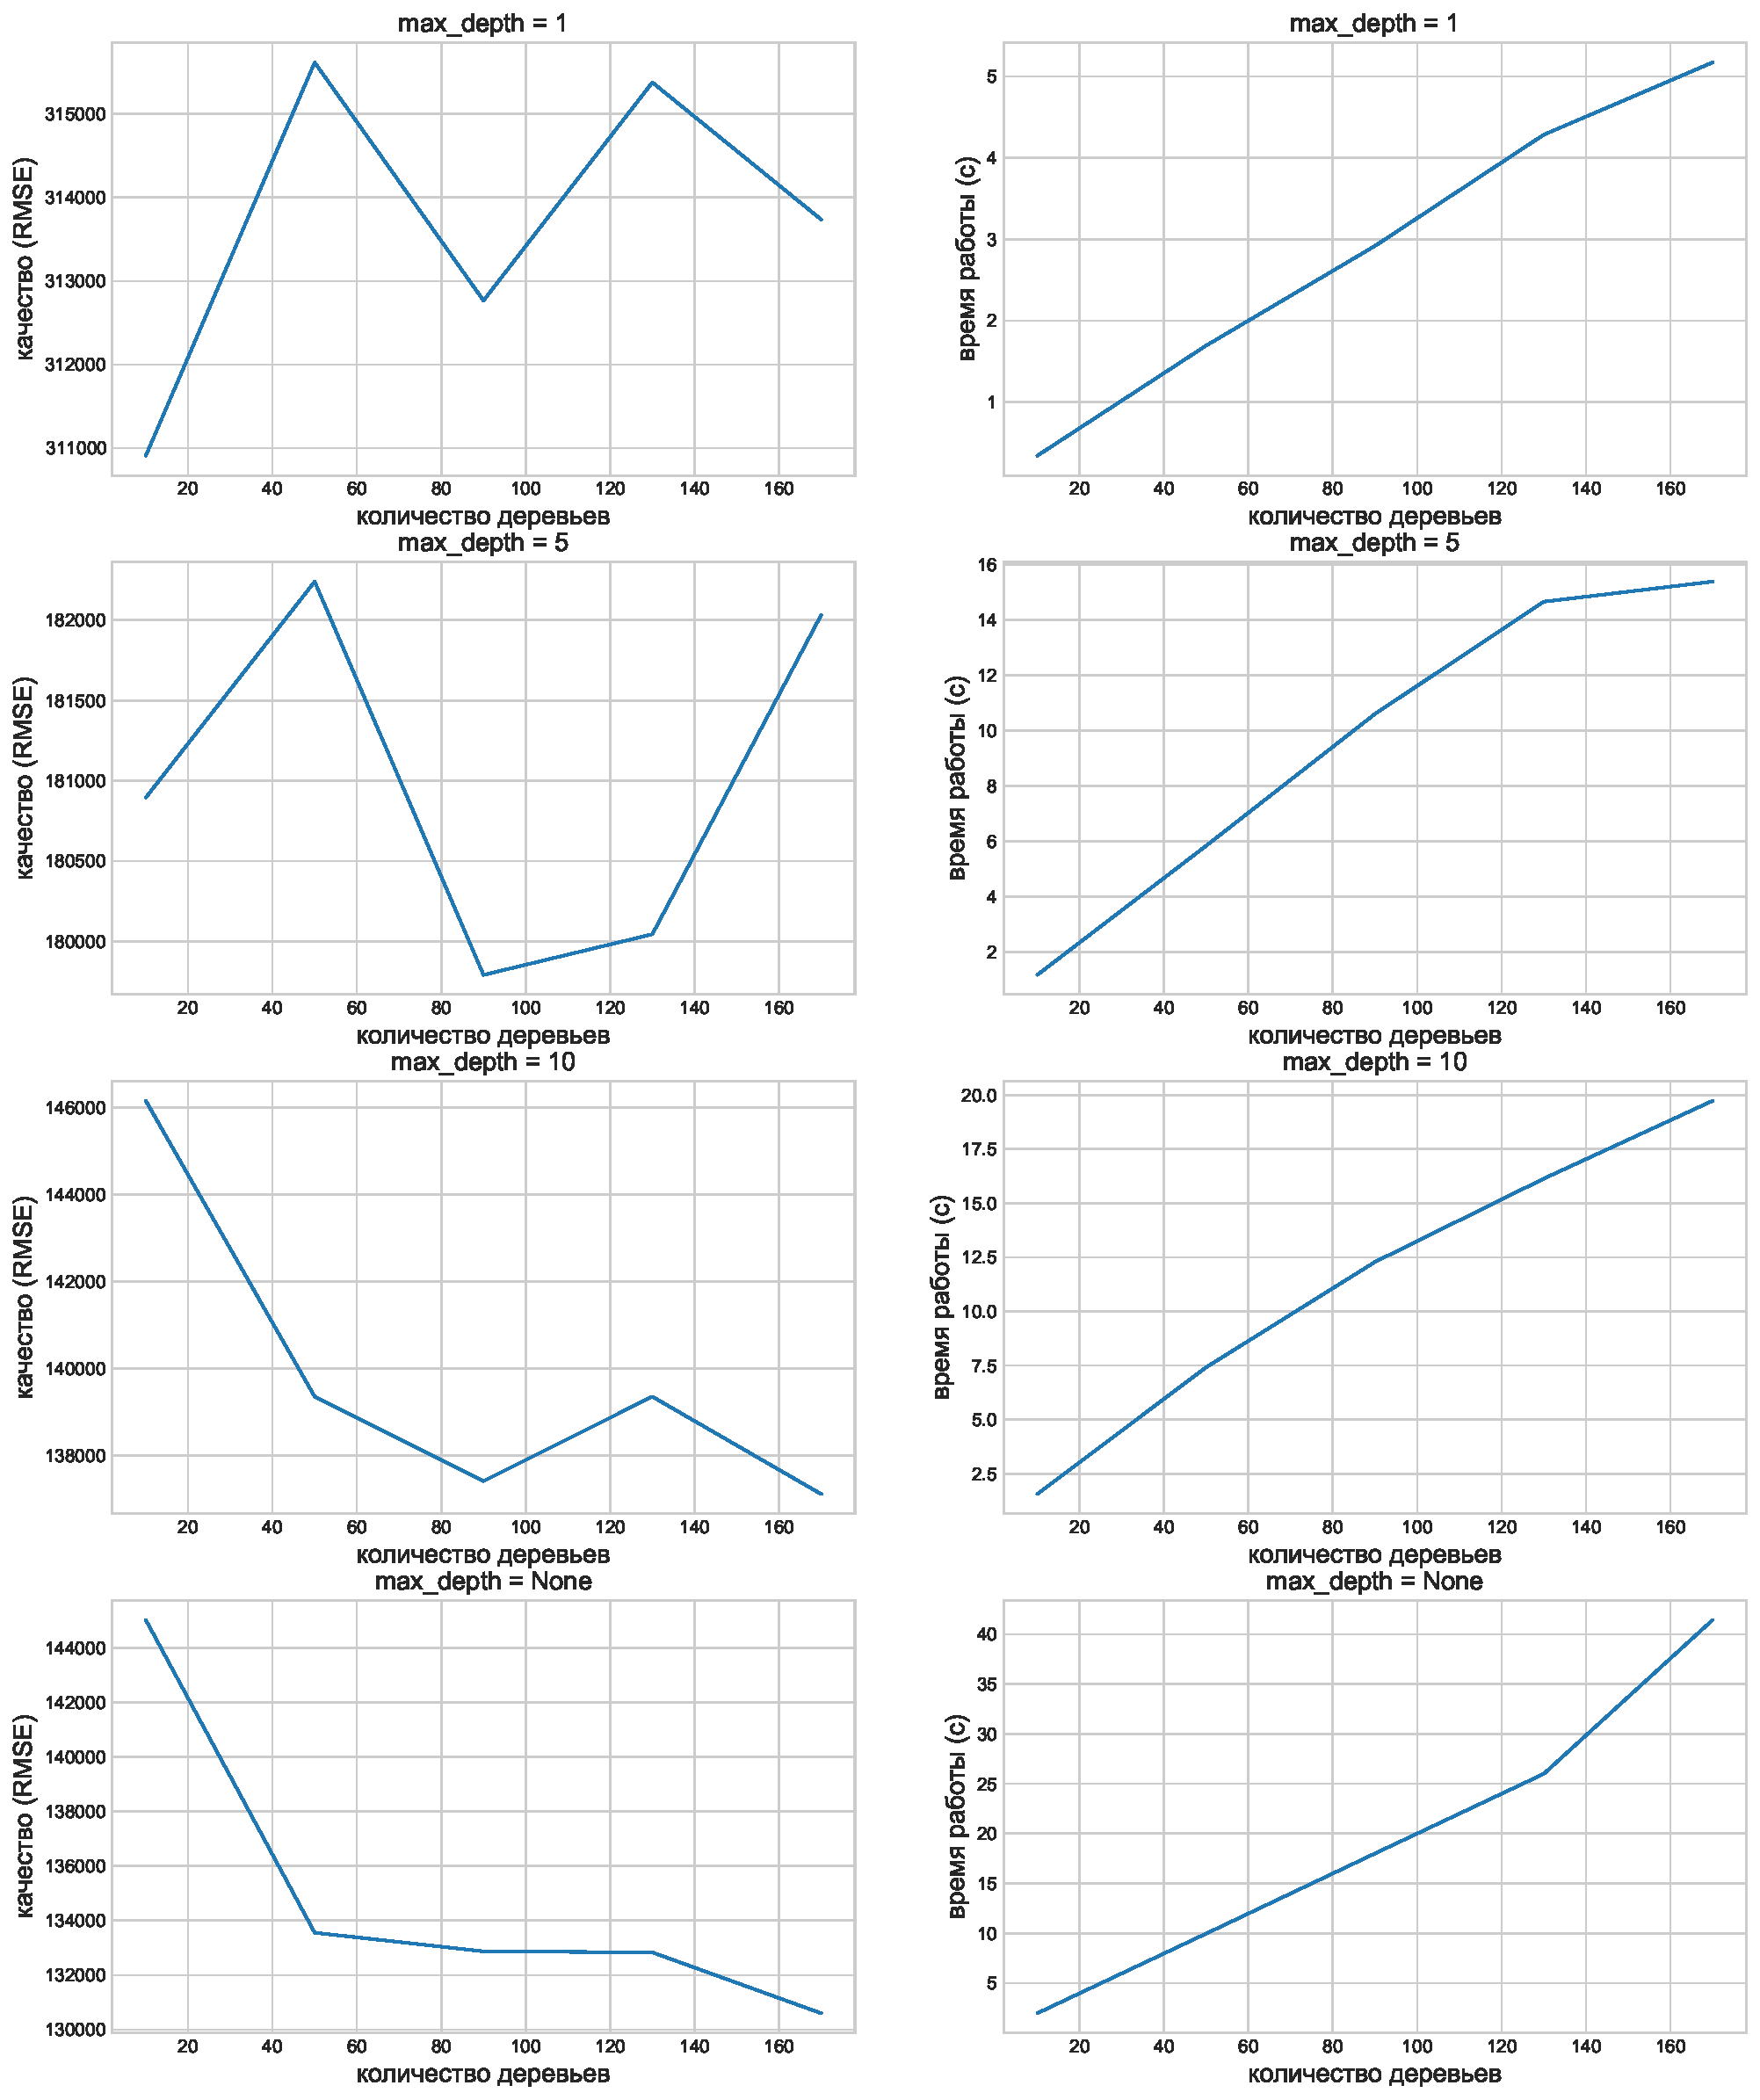
\includegraphics[width=\linewidth]{images/1.2.pdf}
                \end{subfigure}
            \end{figure} \\
            
\subsection{Ограничение глубины деревьев}
При обучении деревьев мы учитываем не их строение, а именно глубину. Так как для каждого дерева подаётся своя сгенерированная обучающая выборка, деревья предсказания делают по-разному и структура их различна. Подстраиваясь под выборку, деревья могут приобретать слишком большую глубину - это плохо сказывается на времени обучения всей модели. K тому же присутствует возможность переобучения. 
Как видно из графиков, глубина деревьев значительно влияет на время обучения модели. Заметим, что после определенного порога количества деревьев, в модели качество перестаёт расти или растёт очень медленно. 
Прослеживается тенденция, что при увеличении глубины деревье качество модели повышается. Проверим это на больших значениях глубин деревьев, выбирая в качестве оптимального значения количества деревьев n\_estimators=90.\\

\begin{figure}[h!]
                \centering
                \begin{subfigure}[b]{1.0\textwidth}
                    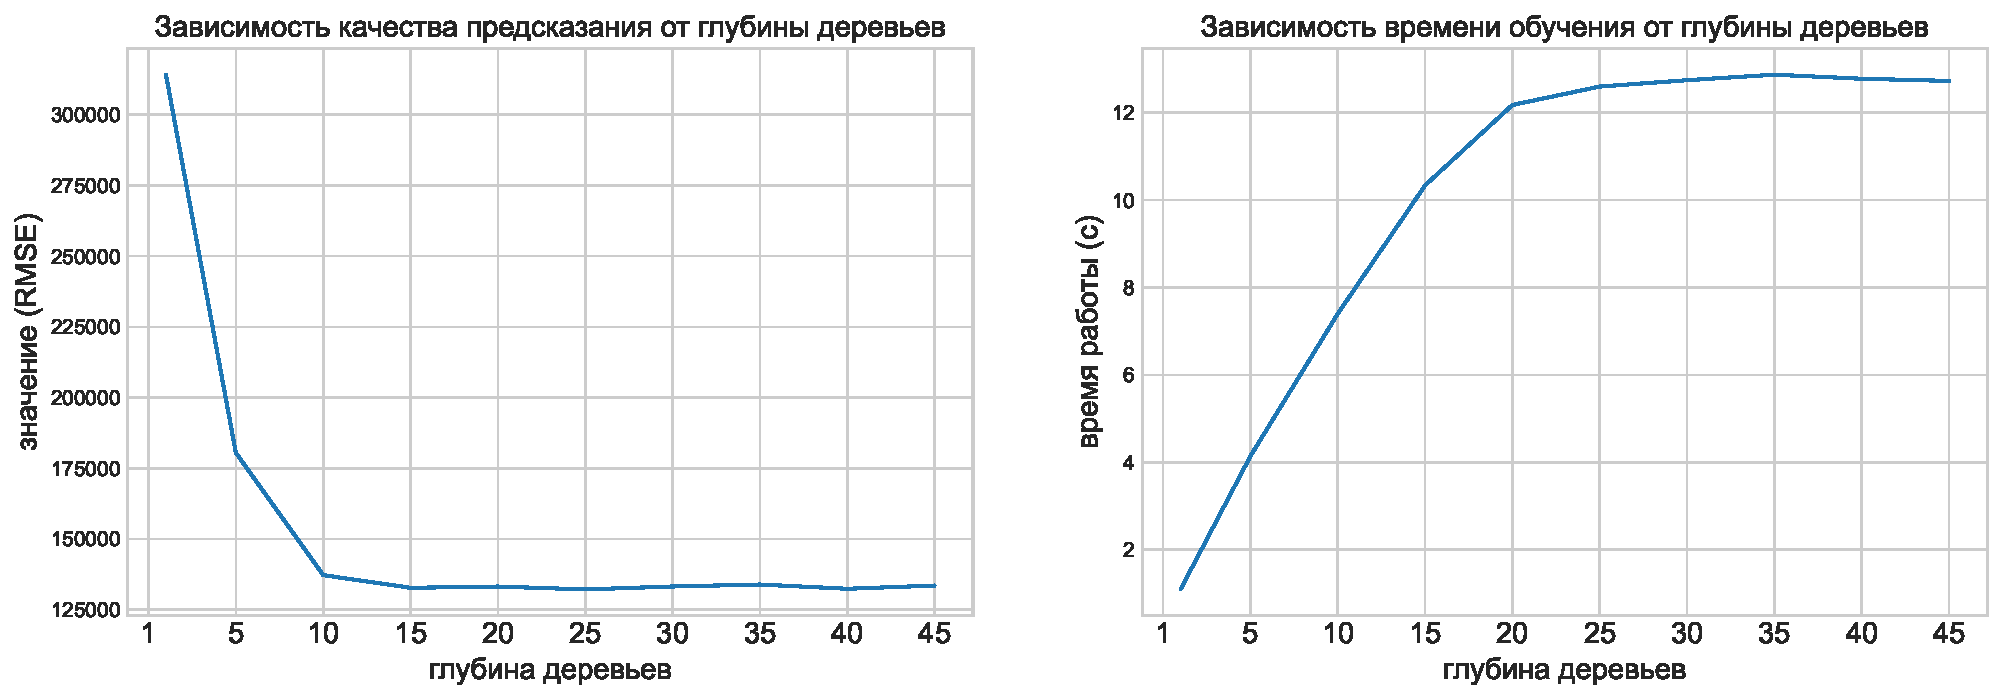
\includegraphics[width=\linewidth]{images/1.2.2.pdf}
                \end{subfigure}
            \end{figure} \\

Время обучения в этот раз линейно зависит от параметра только при значениях глубины, меньших 20, затем оно выходит на "плато". И лучшую точность будут давать более глубокие деревья.

\begin{figure}[h!]
                \centering
                \begin{subfigure}[b]{1.0\textwidth}
                    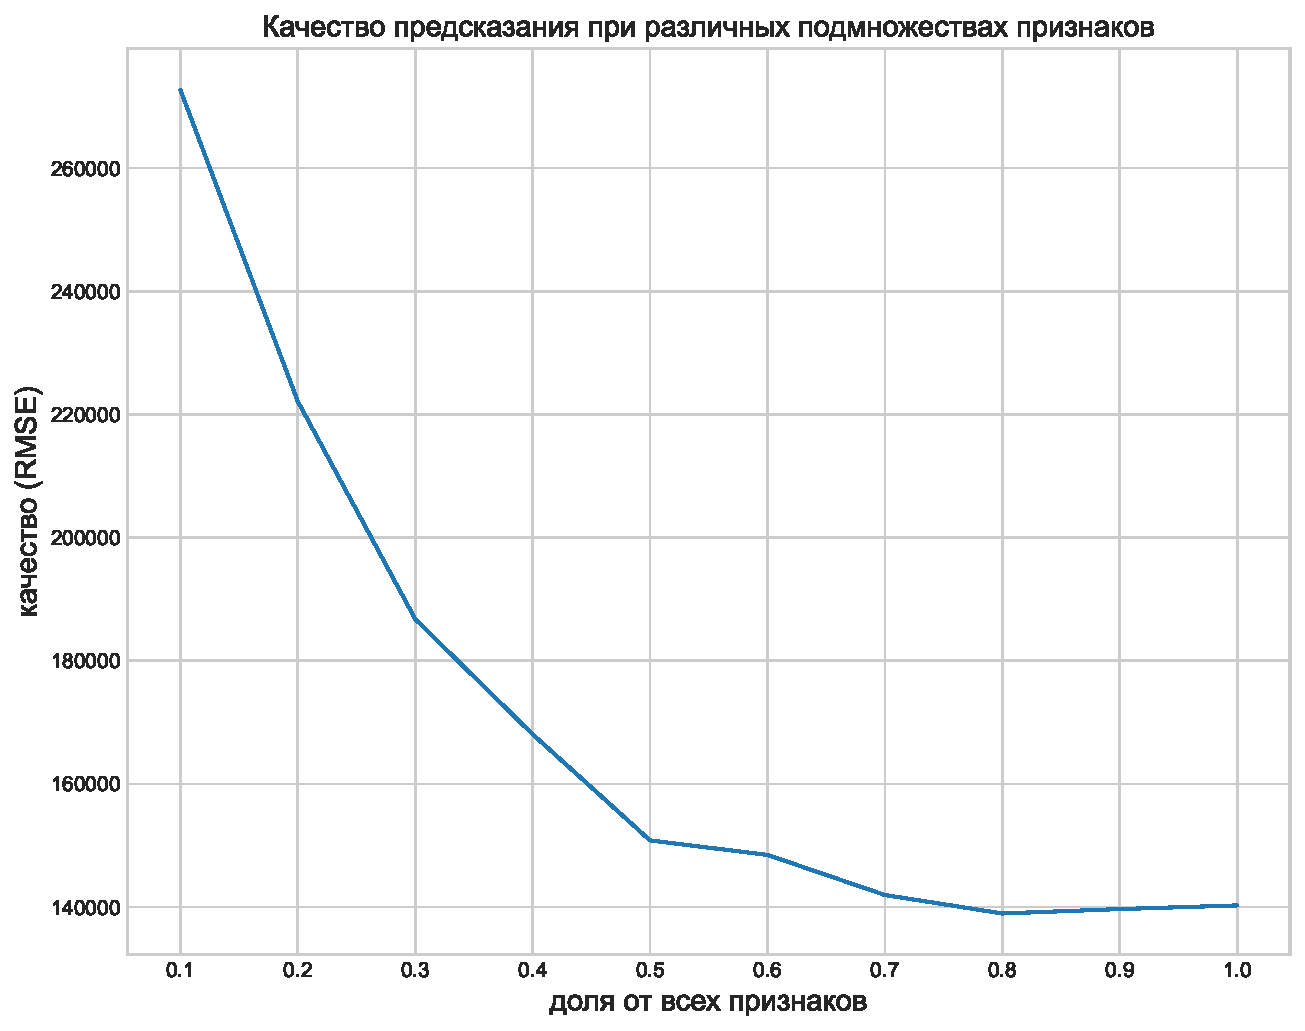
\includegraphics[width=\linewidth]{images/1.3.pdf}
                \end{subfigure}
            \end{figure} \\

\subsection{Изменение признакового пространства}
Здесь исследуем, как размер подмножества признаков влияет на качество предсказания алгоритма. В модели обучаются 90 деревьев с максимальной глубиной 10. 
График выше демострирует зависимость качества предсказания от доли признаков. Результат будет лучше, если каждое дерево будет использовать чуть меньшую информацию об объектах. Каждое дерево упрощает за счёт этого свою структуру, и растёт скорость обучения. Поэтому за оптимальное возьмем количество признаков равное 17.

\section{Модель GradientBoosting}
\subsection{Структура модели}
Данная модель представляет собой композицию некоторого числа базовых алгоритмов, как и в предыдущем случае, в ней будут использованы решающие деревья. Каждое дерево будет вносить свой вклад в общий ответ модели, но делать это будет иным образом по сравнению со случайным лесом. В первой модели деревья строились независимо друг от друга и не могли передавать информаию о совершенных ошибках. Сделаем всё наоборот. Пусть каждое следующее дерево учиться на ошибках предыдущих и пытается эти ошибки исправить. В этом и заключается главная идея этого подхода. Опуская все тонкости реализации, перейдём к исследованию параметров.

\subsection{Влияние числа деревьев на работу модели}
Как и в первой моделе, рассмотрим, каким образом число деревьев в ансамбле влияет на скорость обучения и качество предсказания. Так как деревья обучаются на ошибках предыдущей композиции существует момент, когда увеличение качества прекратится. Насколько рано этот порог наступает, видно из следующих графиков:\\

\begin{figure}[h!]
                \centering
                \begin{subfigure}[b]{1.0\textwidth}
                    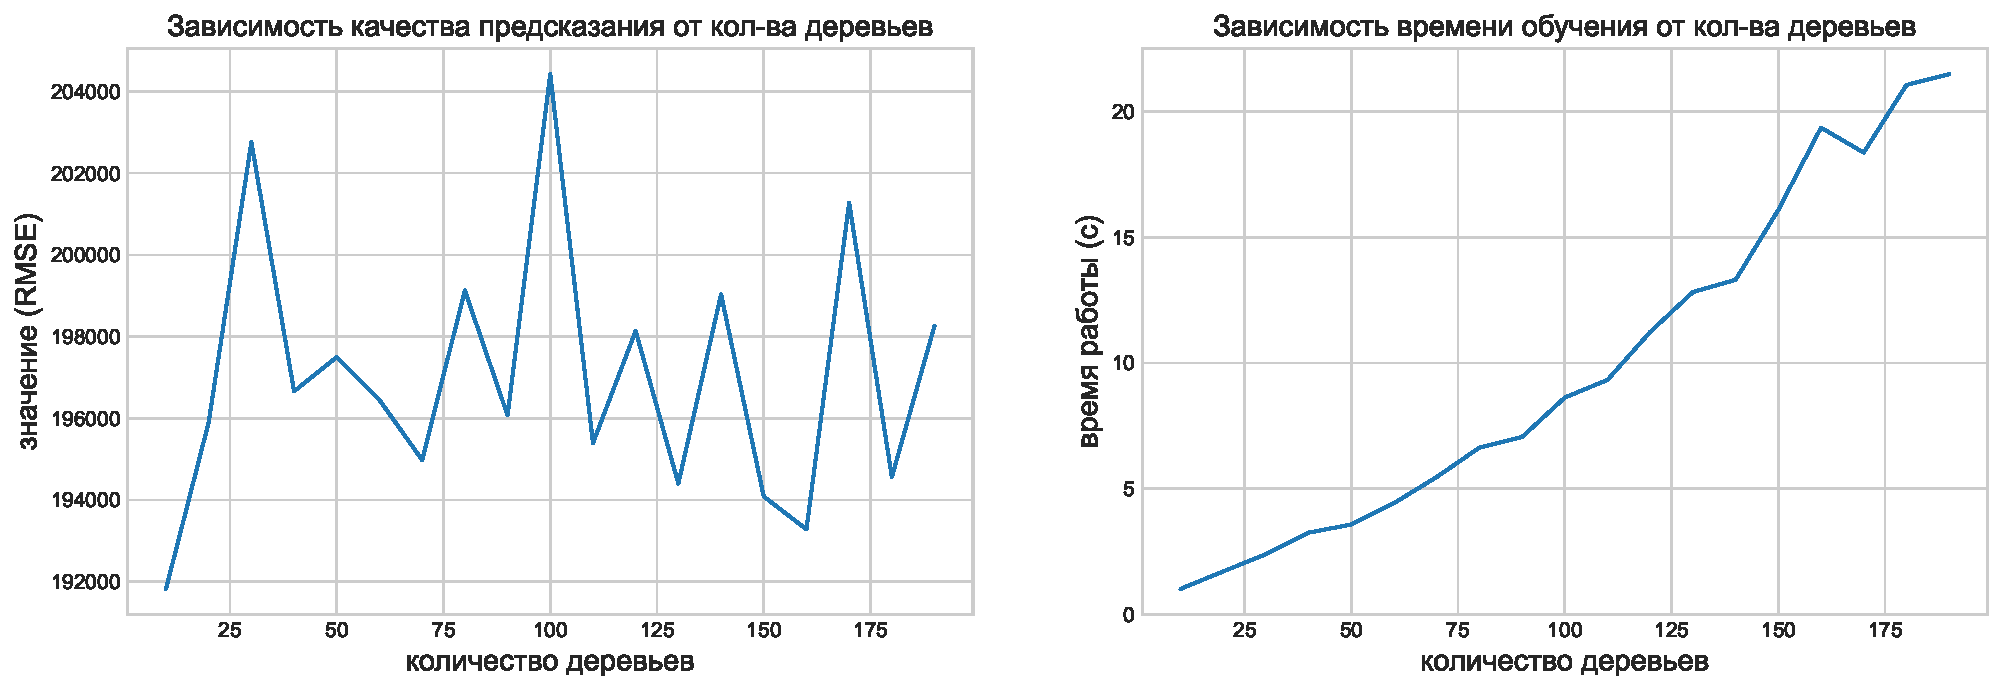
\includegraphics[width=\linewidth]{images/2.1.pdf}
                \end{subfigure}
            \end{figure} \\

Исследование начиналось со значения 10 для количества деревьев. Из графика видно, что увеличение сложности композиции приводит к случайным колебаниям, возможно, искомый порог был пропущен. Проведём тот же эксперимент при количестве деревьев от 1 до 30.

\begin{figure}[h!]
                \centering
                \begin{subfigure}[b]{1.0\textwidth}
                    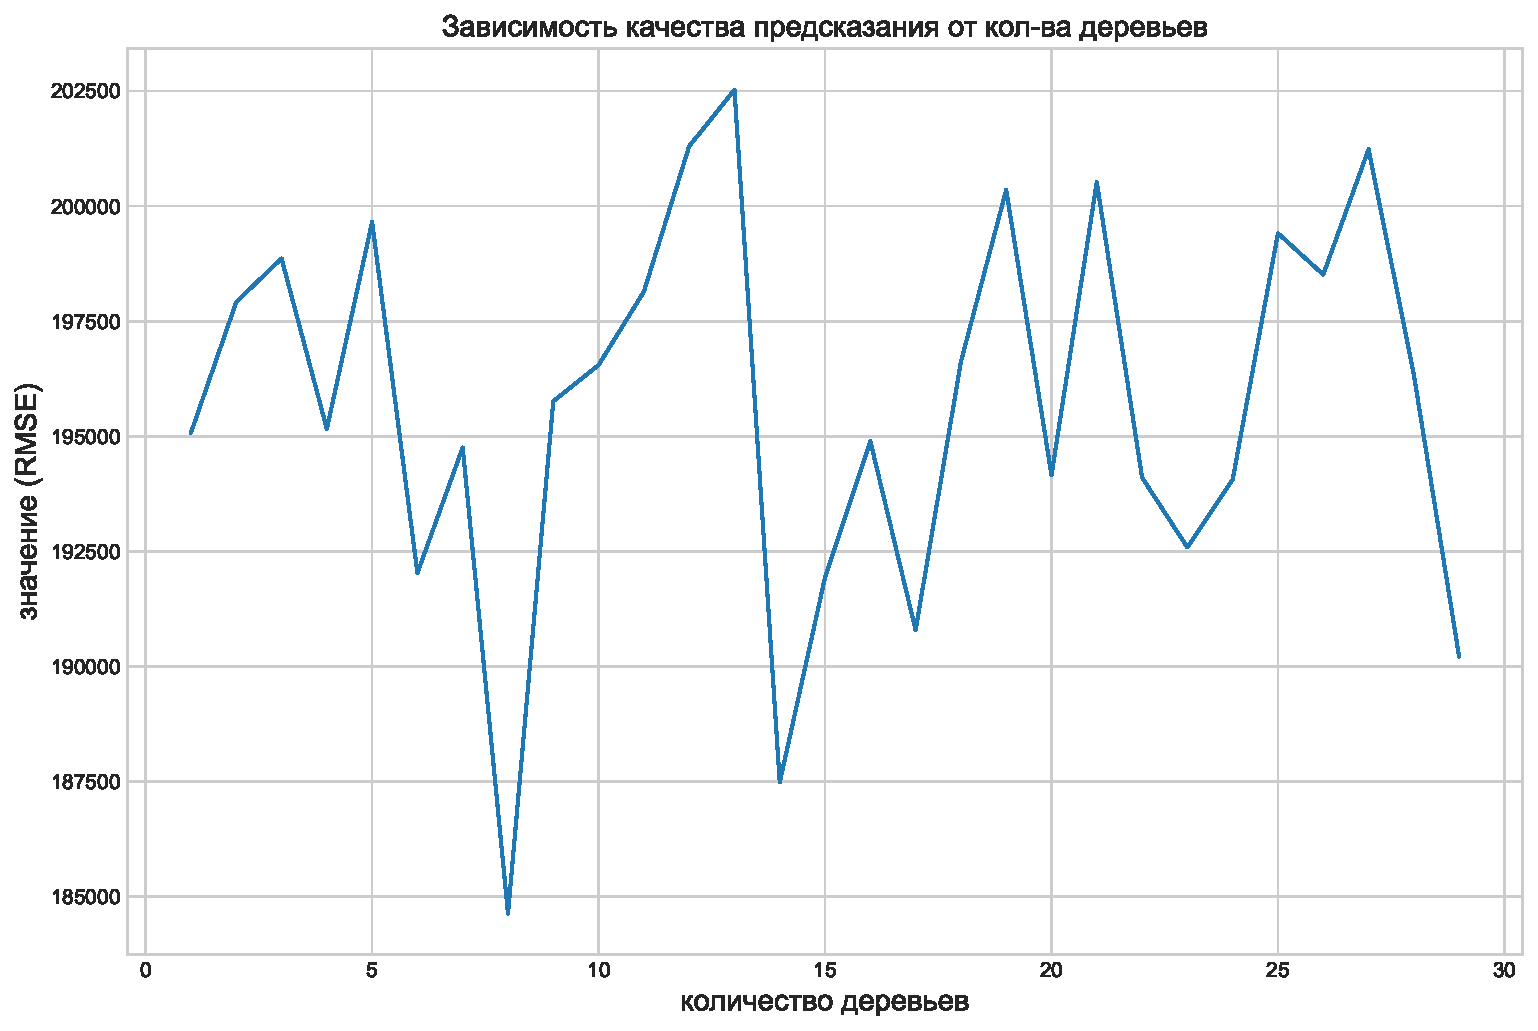
\includegraphics[width=\linewidth]{images/2.1.1.pdf}
                \end{subfigure}
            \end{figure} \\

Исходя из графика, расположенного ниже, лучшее качество достигается при 8 деревьях, убывает и медленно скачками возрастает до значения при 13 деревьях. Потом снова повторяется цикл. Поведение довольно нестандартное и аномальное. Исследуем другие параметры, выяснив, каким образом они могут исправить ситуацию.

\newpage
\subsection{Ограничение глубины деревьев}
Глубина дерева является сильным факторов в вопросе о качестве и времени работы алгоритма, подобно первой модели проведём большое сравнение зависимостей аспектов работы модели при различных ограничениях на глубину дерева.\\

Во всех экспериментах качество ухудшалось с ростом размера композиции. Время работы для различных способов отличается в среднем в несколько раз, чем меньше глубина, тем быстрее строятся деревья. Во всех случаях наилучшее качество достигалось при минимальном числе деревьев, причём лучшее из них - при максимальной глубине деревьев, равной 5. По-прежнему выгоднее брать небольшое число деревьев (до 30).
\newpage

\begin{figure}[h!]
                \centering
                \begin{subfigure}[b]{1.0\textwidth}
                    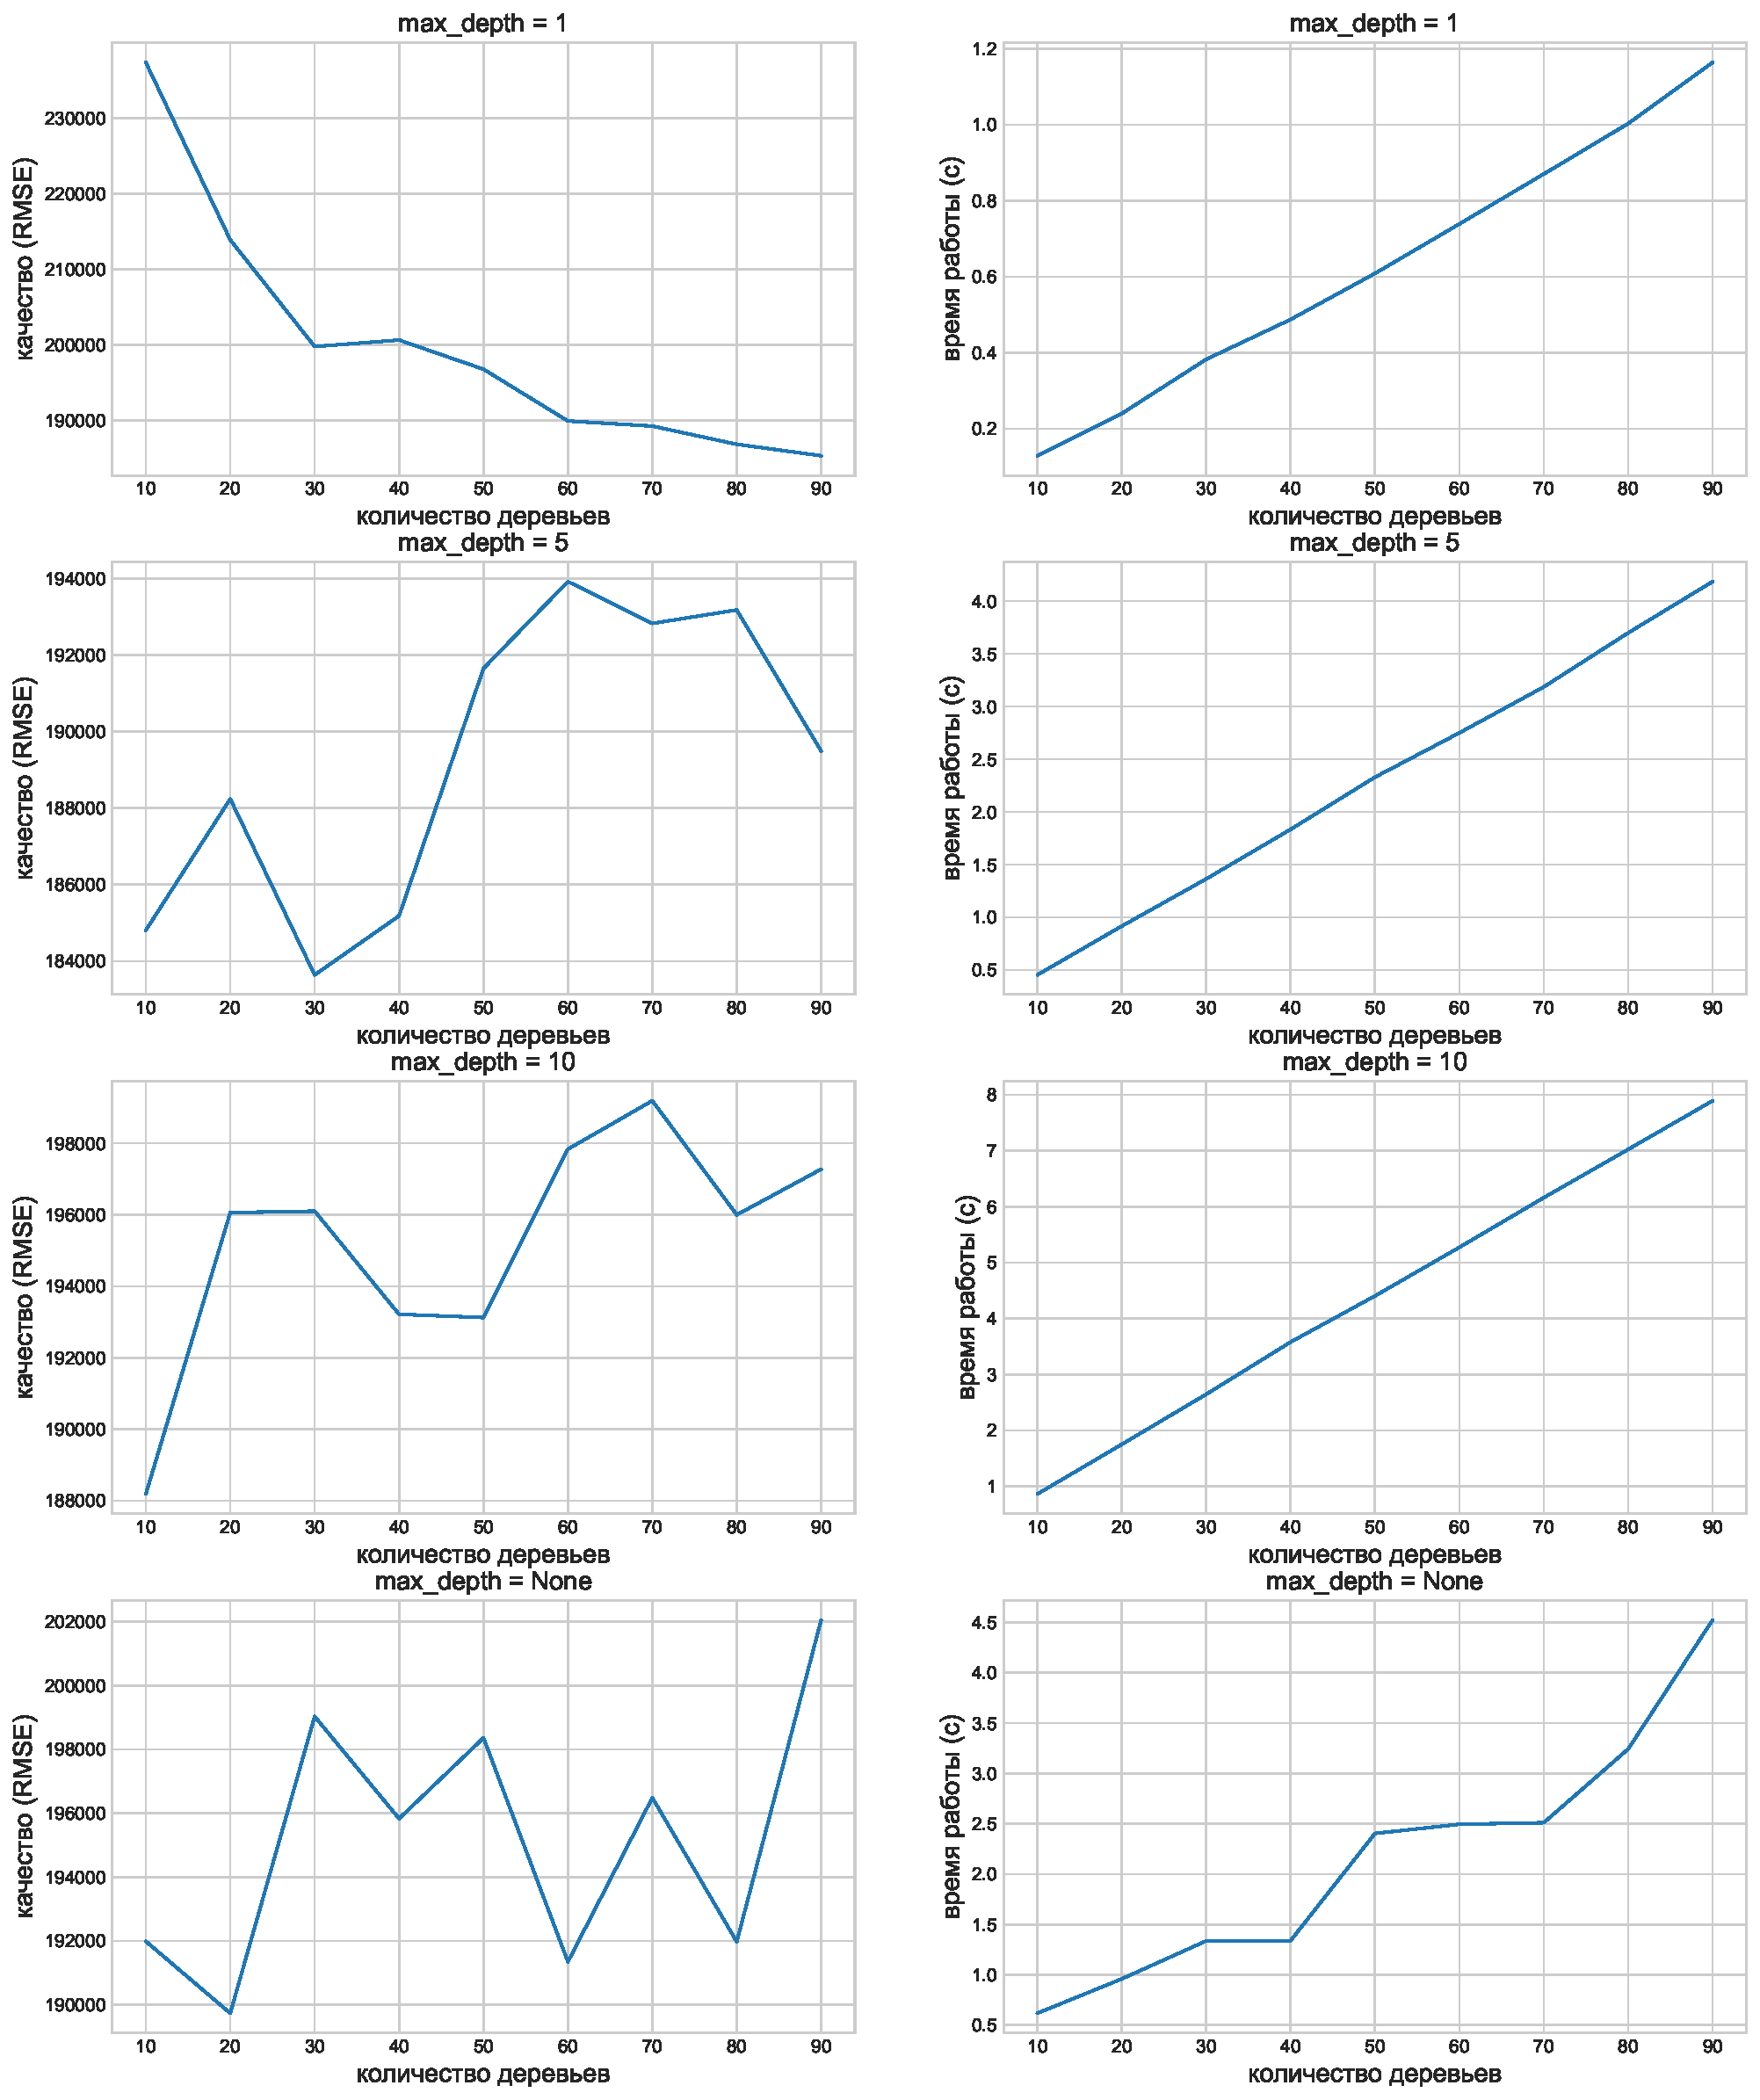
\includegraphics[width=\linewidth]{images/2.2.pdf}
                \end{subfigure}
            \end{figure}

\subsection{Изменение признакового пространства}
Так вышло, что модель с максимально《короткими» деревьями показывала наилучшие результаты. Подобная глубина означает, что дерево осуществляет прогноз на основании нескольких признаков. Их дерево выбирает из всего множества признаков, у алгоритма имеется после дополнительная информация об объекте, которая является для него излишней. Попробуем увеличить количество используемых признаков, но и ограничить количество рассматриваемых признаков для построения каждого из деревьев.
Даже в таком случае моделе проще делать качественные предсказания при как можно меньшем наборе признаков. Можно предположить, что среди признаков есть очень информативный, попадание которого в признаковое пространство сильно влияет на качество - это видно из «падений» графика вниз.

\begin{figure}[h!]
                \centering
                \begin{subfigure}[b]{1.0\textwidth}
                    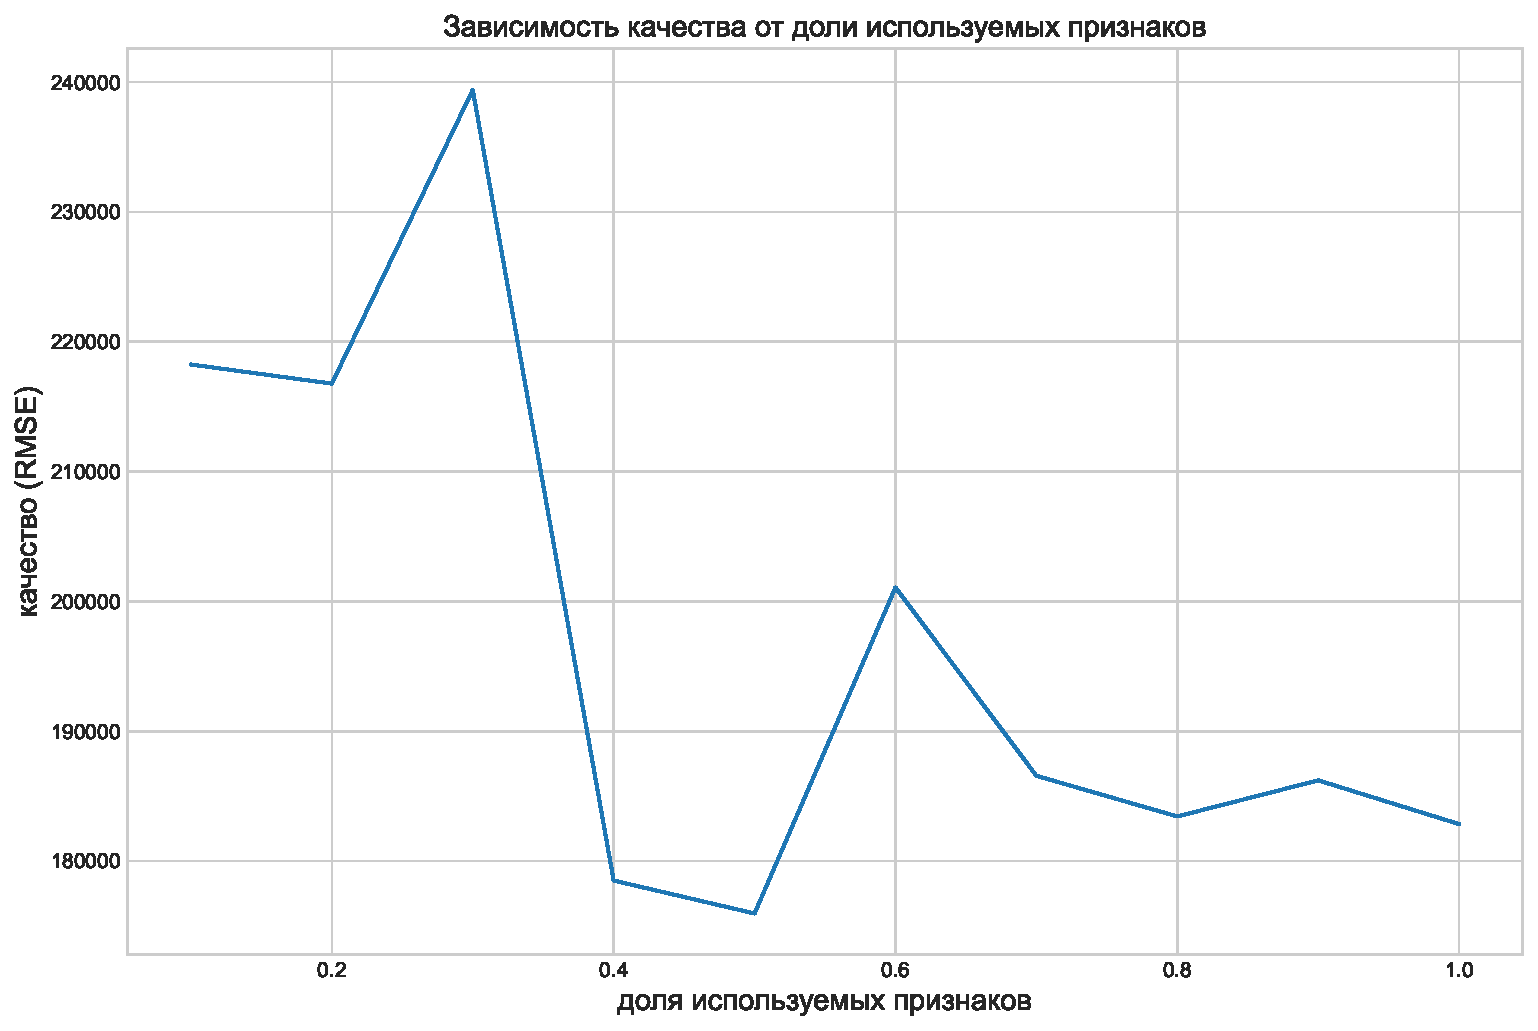
\includegraphics[width=\linewidth]{images/2.3.pdf}
                \end{subfigure}
            \end{figure} \\

\begin{figure}[h!]
                \centering
                \begin{subfigure}[b]{1.0\textwidth}
                    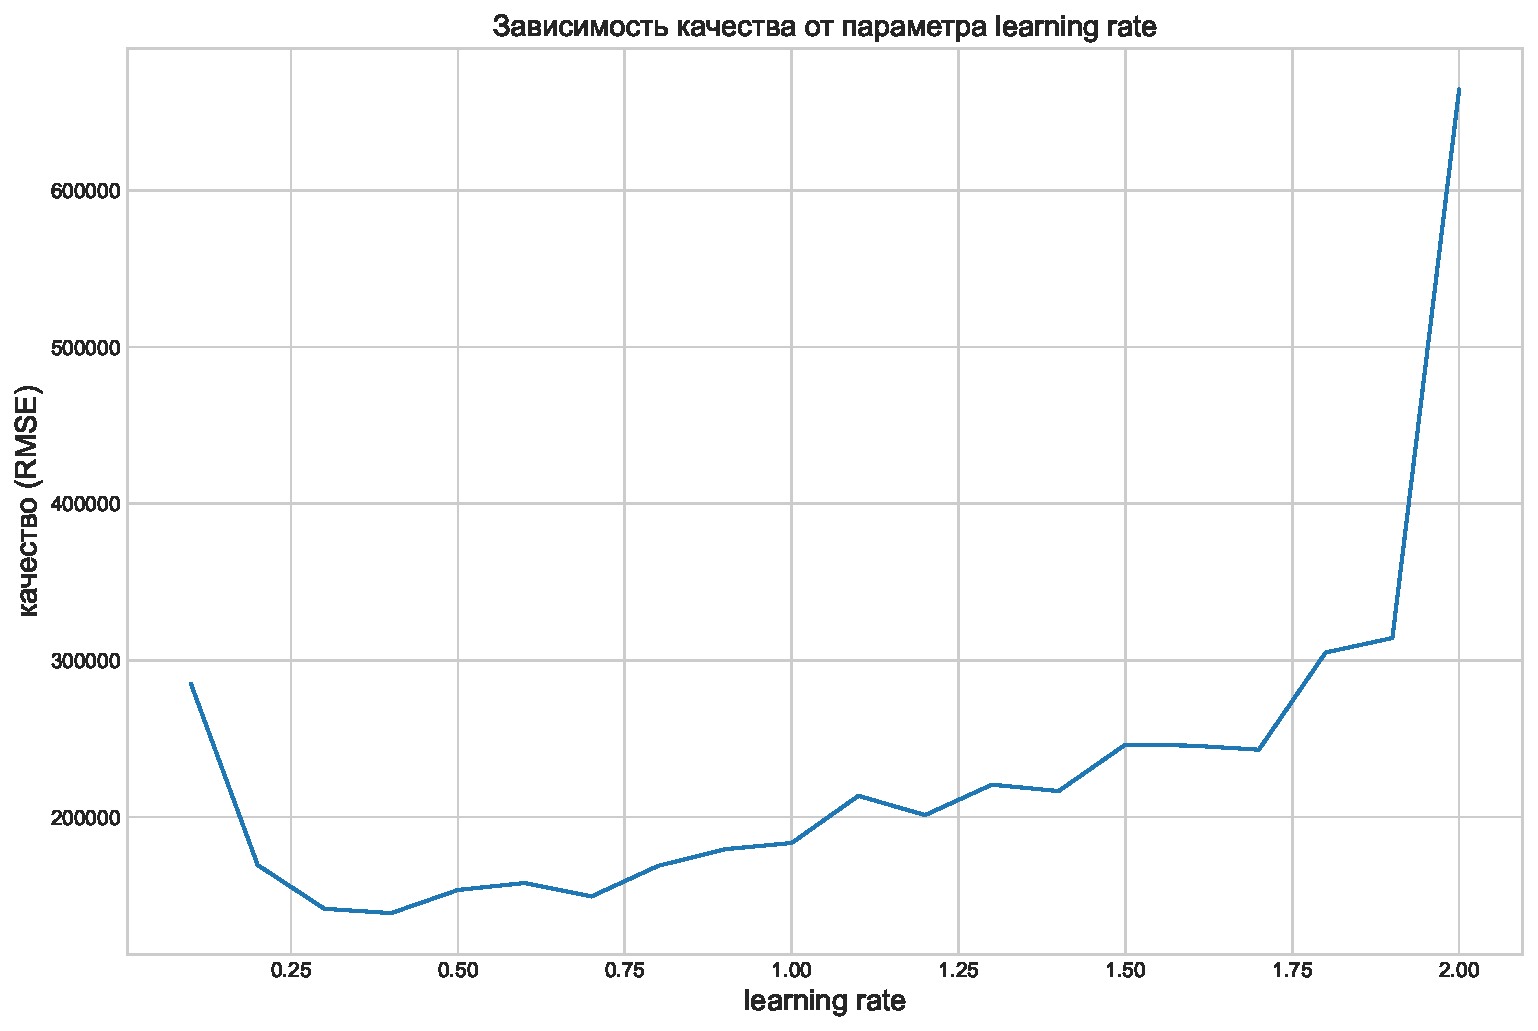
\includegraphics[width=\linewidth]{images/2.4.pdf}
                \end{subfigure}
            \end{figure} \\



\subsection{Вклад каждого алгоритма в ансамбль}
Выше было выяснено, что меньшее число деревьев даёт лучший результат. Каждое дерево добавляется в ансамбль с некотором коэфициентом $\gamma$, который находится из соответствующей оптимизационной задачи. Попробуем уменьшить вклад каждого дерева в общий прогноз, домножая этот коэффициент на параметр learning\_rate.


Модель с количеством деревьев - 10, их максимальной глубиной - 5, получила лучшее качество при параметре learning\_rate равным ~0.4. Вклад каждого дерева уменьшался более, чем в 2 раза. Чем больше в композиции деревьев, тем меньше будет значение параметра и учёт прогноза этого дерева в общем прогнозе.

\section{Вывод}
В ходе работы были реализованы алгоритмы предсказания RandomForest и GradientBoosting на решающих деревьях. Алгоритм случайного леса выдавал ожидаемые результаты: при увеличении количества деревьев росло качество и время работы, но не бесконечно. С очень большим количеством деревьев затрачиваемое время работы становится слишком большим и появляется риск переобучения. Имеет смысл проводить тонкую настройку деревьев, например, регулировать их максимальную глубину, признаковое пространство, на котором они обучаются, чтобы получить результат более высокого уровня с точки зрения качества и времени работы. Метод градиентного бустинга над решающими деревьями на протяжении всех экспериментов выдавал неоднозначные результаты. Увеличение размера ансамбля слабо влияло на качество, в некоторых местах даже ухудшало, исходя из экпериментов, можно вообще сделать вывод, что, чем меньше деревьев задействованы в работе, тем лучше. В случае всего лишь одного дерева метод вырождается в одно решающее дерево, причём и глубину брать маленькую также выгоднее, чем большую. А это равносильно тому, что мы осуществляем предсказание для объекта, основываясь лишь на значении одного признака: больше оно или меньше определенного порога для этого признака. В этих случаях регулирование остальных параметров не имеет большого смысла. Несмотря на все замечания второй метод работает чуть лучше первого. И возникает вопрос: не лучше ли использовать одно тонко настроенное дерево? Теоретически нет, не лучше. Проблема может заключаться в отсутствии предобработки входных данных. Никак не были исследованы признаки, их полезность и влияние на работу методов. Также были проигнорированы возможные объекты-выбросы, которые могут плохо влиять на предсказательную способность алгоритмов.

При сравнении алгоритмов с точки зрения различных машинных оптимизаций можно выявить следующее различие между исследованными моделями: модель случайного леса может тренировать деревья параллельно независимо друг от друга - это даст значительное ускорение, градиентный бустинг распараллеливание может производить только на этапе обучения конкретного базового алгоритма, так как между собой алгоритмы «связаны» последовательно.

\end{document}